% include all necessary latex libraries
\documentclass[aspectratio=169,presentation]{beamer}
\usetheme{Boadilla}
\useinnertheme{default}

% -- locale-setup --------------------------------------------------------------

\usepackage[utf8]{inputenc}
\usepackage[T1]{fontenc}
\usepackage[ngerman]{babel}
\usepackage{lmodern}
\usepackage[locale=DE, mode=math, list-final-separator={ oder },
            range-phrase={ bis }, scientific-notation=false, 
            group-digits=integer] {siunitx}

% -- package-includes ----------------------------------------------------------

\usepackage{tikz}
\usepackage{xcolor}
\usetikzlibrary{positioning,automata,matrix,arrows.meta,fit}
\usepackage{graphicx} % including images
\usepackage[font=small,labelfont=bf]{caption} % captions of tables and figures

% -- listing setup -------------------------------------------------------------

\usepackage{listings}
\definecolor{pblue}{rgb}{0.13,0.13,1}
\definecolor{pgreen}{rgb}{0,0.5,0}
\definecolor{pred}{rgb}{0.9,0,0}
\definecolor{pgrey}{rgb}{0.46,0.45,0.48}
\definecolor{javared}{rgb}{0.6,0,0} % for strings
\definecolor{javagreen}{rgb}{0.25,0.5,0.35} % comments
\definecolor{javapurple}{rgb}{0.5,0,0.35} % keywords
\definecolor{javadocblue}{rgb}{0.25,0.35,0.75} % javadoc

\lstset{language=vhdl,
	basicstyle=\ttfamily,
	keywordstyle=\color{javapurple}\bfseries,
	stringstyle=\color{javared},
	commentstyle=\color{javagreen},
	morecomment=[s][\color{javadocblue}]{/**}{*/},
	tabsize=2,
	showspaces=false,
	showstringspaces=false
}

% -- custom commands -----------------------------------------------------------

% just prints given text in large text and on empty frame.
\newcommand{\sectionframe} [1] {
	\begin{frame}
		\vfill
		\Huge
		\centering
		\usebeamercolor[fg]{title}
		#1
		\vfill
		\par
	\end{frame}
}

% wrapper-command to make pretty title takes
% 1=short-title 2=long-title 3=terminnumber 4=date
\newcommand{\maketitlepage} [5] {
  \title[#1]{#2}
  \subtitle{Termin #3}
  \date{#4}
  \author[Jakob Otto]{Jakob Otto}
  \institute{HAW Hamburg}
  \subject{#1}
  \pgfdeclareimage[height=0.5cm, width=1.3cm]{university-logo}{#5}
  \logo{\href{https://www.haw-hamburg.de}{\pgfuseimage{university-logo}}}
  \begin{frame} {}
    \titlepage
  \end{frame}
}

% draws a link symbol
\newcommand{\externalLink} {
  \tikz[x=1.2ex, y=1.2ex, baseline=-0.05ex]{
    \begin{scope}[x=1ex, y=1ex]
      \clip (-0.1,-0.1) 
        --++ (-0, 1.2) 
        --++ (0.6, 0) 
        --++ (0, -0.6) 
        --++ (0.6, 0) 
        --++ (0, -1);
      \path[draw, 
        line width = 0.5, 
        rounded corners=0.5] 
      (0,0) rectangle (1,1);
    \end{scope}
      \path[draw, line width = 0.5] (0.5, 0.5) 
        -- (1, 1);
    \path[draw, line width = 0.5] (0.6, 1) 
      -- (1, 1) -- (1, 0.6);
  }
}

% Adds a circled number -> Looks better than the default
\newcommand{\circled} [1] {
  \tikz[baseline=(char.base)]{
    \node[shape=circle,draw,inner sep=2pt, text centered, text width = .2cm] (char) {#1};
  }
}

% -- extra includes go here ----------------------------------------------------
% ...

\begin{document}
  \maketitlepage {CE Tutorium} {Tutorium zu\\Computer-Engineering\\im SS19} {4} 
                 {10. Oktober 2019} {../presentation-template/figs/logo-haw-2017}

  %-----------------------------------------------------------------------------
  %	Ablauf
  %-----------------------------------------------------------------------------
  \section{Ablauf}
  \begin{frame}{Ablauf}
    \begin{columns}
      \column{0.4\textwidth}
      \begin{itemize}
        \item Begrüßung
        \begin{itemize}
          \item Wer bin ich?
          \item Was stelle ich mir vor?
          \item Was stellt ihr euch vor?
        \end{itemize}
        \item Kurze Wiederholung
        \item Praktikum
        \begin{itemize}
          \item 7-Segment-Display
          \item Shiftregister
          \item Tick-generator
          \item Lookup table
        \end{itemize}
      \end{itemize}
      \column{0.6\textwidth}
        \begin{center}
          
\includegraphics[width=.6\textwidth]{../presentation-template/figs/kratzen}
        \end{center}
    \end{columns}
  \end{frame}

  %-----------------------------------------------------------------------------
  %	Begrüßung
  %-----------------------------------------------------------------------------

  \section{Begrüßung}
  \begin{frame} {Wer bin ich?}
    \begin{columns}
      \column{0.6\textwidth}
        \begin{itemize}
          \item Jakob Otto
          \item Gerade dabei den Bachelor zu schreiben
          \item C++, Internet, Distributed Systems
          \item Entsprechend oft bei der Inet-Group zu finden
        \end{itemize}
      \column{0.4\textwidth}
        \begin{center}
          \href{https://inet.haw-hamburg.de}{
\includegraphics[width=.4\textwidth]
               {figs/inet_logo.png}\externalLink}
        \end{center}
        \begin{center}
          \href{https://actor-framework.org}{
\includegraphics[width=.4\textwidth]
               {figs/caf_logo.png}\externalLink}
        \end{center}
    \end{columns}
  \end{frame}

  \begin{frame} {Meine Vorstellung fürs Tutorium}
    \begin{block} {Meine Ziele sind}
      \begin{itemize}
        \item Euch durchs Praktikum zu bringen
        \item Verständnisfragen klären
        \item Persönliche Hilfe anbieten
      \end{itemize}
    \end{block}
    \begin{exampleblock} {No worries.}
      Frontalvorträge sind nicht meins
    \end{exampleblock}
  \end{frame}

  \sectionframe{Was wollt ihr??}

  %-----------------------------------------------------------------------------
  %	Praktkumsaufgabe
  %-----------------------------------------------------------------------------

  \sectionframe{\href{https://users.informatik.haw-hamburg.de/~schafers/LOCAL/S19W_CE/Aufgabenzettel_Nr1_v18.pdf}
               {Aufgabenzettel \externalLink}}

  %-----------------------------------------------------------------------------
  %	Kurze Wiederholung UCF
  %-----------------------------------------------------------------------------

  \section{Kurze Wiederholung}
  \begin{frame} [fragile] {kurze Wiederholung (UCF)}
    \begin{block} {UCF-File}
      \begin{itemize}
        \item mappt ein- und Ausgänge auf pins
        \item Format:
        \begin{lstlisting}
  NET <port-name> LOC = <pin>;
        \end{lstlisting}
        \item Als Beispiel:
        \begin{lstlisting}
  NET "clk"		LOC = "V10";
        \end{lstlisting}
      \end{itemize}
    \end{block}
  \end{frame}

  \begin{frame} [fragile] {Woher die Infos?}
    \begin{block} {}
      \begin{itemize}
        \item Normalerweise aus irgendwelchen Datenblättern..
        \item Hier: Aus der 
              \href{https://users.informatik.haw-hamburg.de/~behn/pub/CEP/FPGA_CE Board.pdf}
                   {\color{red}{CE\underline{ }Board-Doku \externalLink}}
        \item Weitere Doku zum Nexys2-board gibts 
              \href{http://users.informatik.haw-hamburg.de/~schafers/LOCAL/S19S_CE/DOCU/OLD Digilent Nexys2 Board Reference Manual.pdf}
                   {\color{red}{hier \externalLink}}
      \end{itemize}
    \end{block}
  \end{frame}

  %-----------------------------------------------------------------------------
  %	Sieben-Segment-Display
  %-----------------------------------------------------------------------------

  \begin{frame} {Sieben-Segment Display (I)}
    \begin{block} {Besonderheiten bei unserem Package}
      \begin{itemize}
        \item Individelle Anoden
        \item Gemeinsame Kathode
      \end{itemize}
    \end{block}
  \end{frame}

  \section{7-Segment Display}
  \begin{frame} {Sieben-Segment Display (II)}
      \begin{center}
        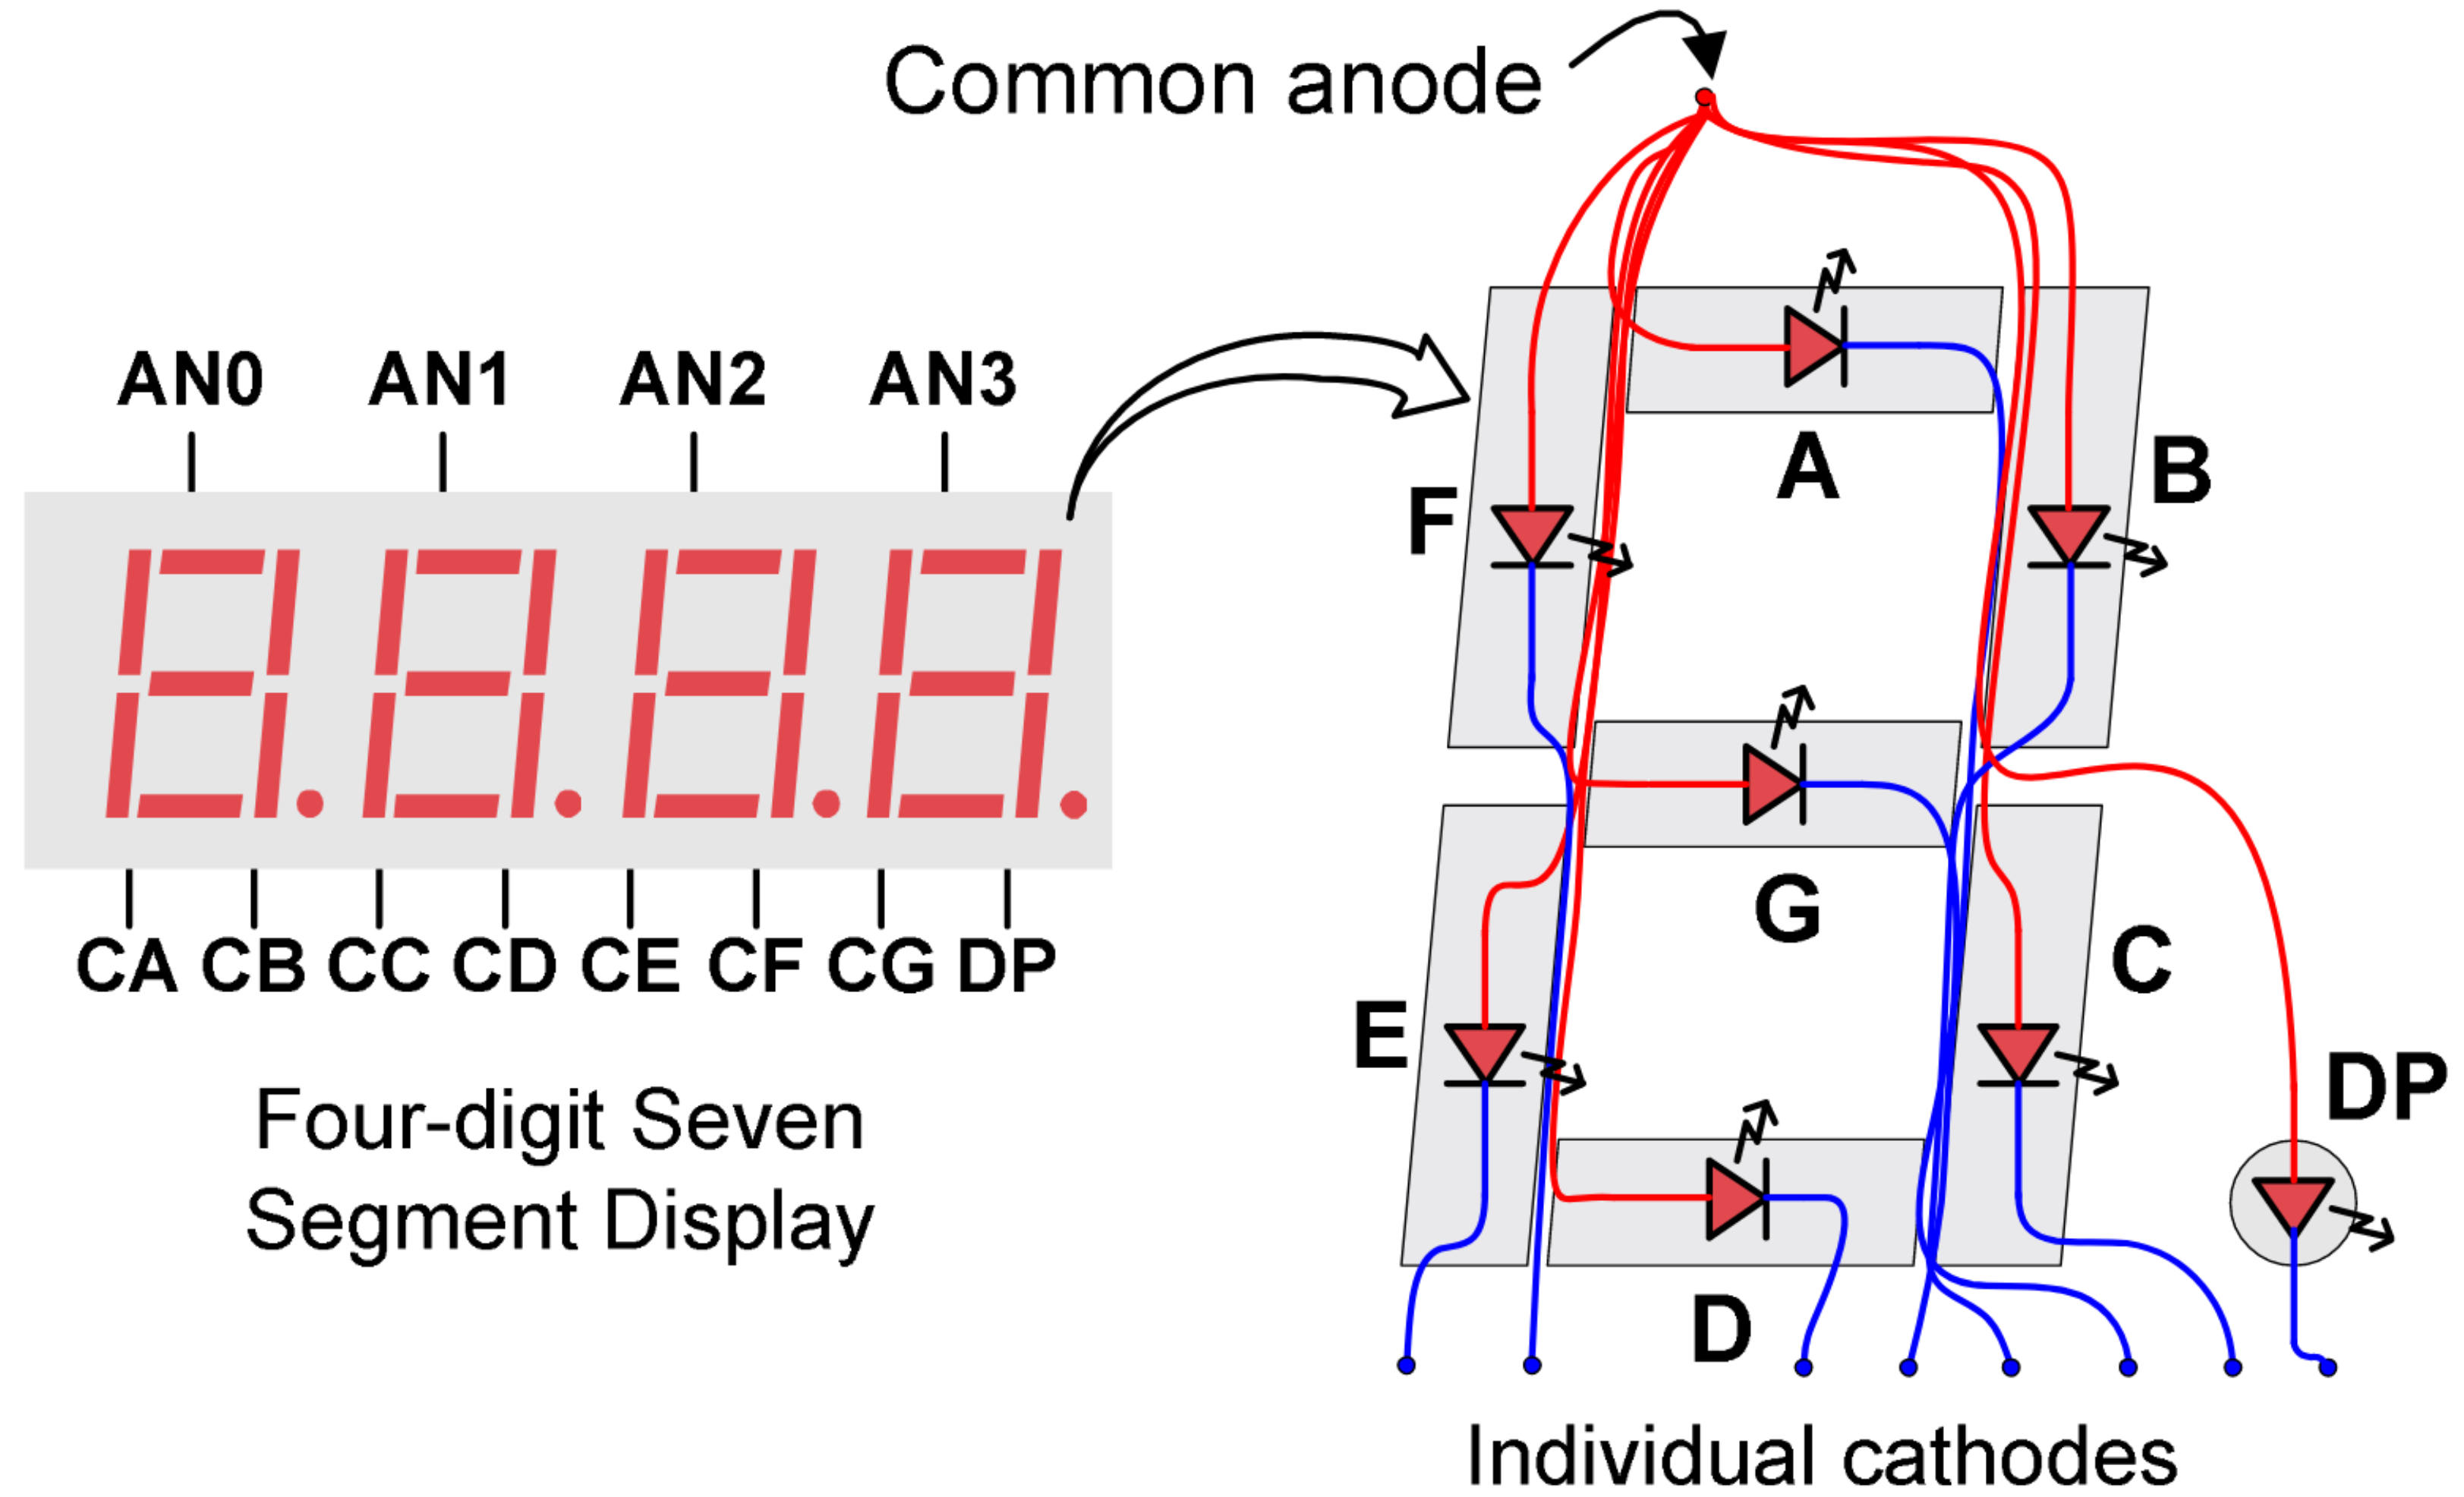
\includegraphics[width=0.8\textwidth]{figs/7seg_display.png}
      \end{center}
  \end{frame}

  %-----------------------------------------------------------------------------
  %	Shiftregister
  %-----------------------------------------------------------------------------

  \section{Shiftregister}
  \begin{frame} {Shiftregister (I)}
    \begin{block} {Verschiedene Zahlen Anzeigen}
      \begin{itemize}
        \item Anoden müssen zyklisch angewählt werden
        \item Zyklisches-Shiftregister passt
        \item Dadurch werden nacheinander die einzelnen Anoden durchgeschaltet.
      \end{itemize}
    \end{block}
  \end{frame}

  \begin{frame} [fragile] {Shiftregister (II)}
    \begin{center}
      \begin{tikzpicture}[>=Stealth,
        scale=2,
        font=\ttfamily,
        bits/.style={draw, minimum size=14mm},
        register/.style={matrix of nodes,nodes={bits},
        column sep=-\pgflinewidth, 
        row sep=0.5mm, nodes in empty cells,
        row 1/.style={nodes={draw=none, minimum size=1cm}},
        }]
        
        \matrix[register, label=below:RLA] (RLA) {
        3 & 2 & 1 & 0\\
        |(3)|&|(2)|&|(1)|&|(0)|\\};
        
        \foreach \i in {0,...,3}
            \draw[->] ([xshift=1mm]\i.east)--++(180:4mm);
        \draw[->] (3.west)--++(180:3mm);
        \draw (3.west)--++(180:1cm)|-(RLA.north)-|([xshift=1cm]0.east)--(0.east);
      \end{tikzpicture}
    \end{center}
  \end{frame}

  \begin{frame} [fragile] {Shiftregister (III)}
    \begin{lstlisting}
  sequlo:
  process (clk) is
  begin
    -- ...
  end process sequlo;

  shift:
  process(rot_cs) is 
  begin
    -- shift reg and append MSB as LSB
    reg_ns <= reg_cs(reg_cs'left-1 downto 0) & reg_cs(reg_cs'left);
  end process shift;
    \end{lstlisting}
    
    \begin{alertblock} {}
      shiftregister sollte mit \grqq{}1110\grqq{} initialisiert werden!\\
      $\rightarrow$ Anode ist low-aktiv
    \end{alertblock}
  \end{frame}

  %-----------------------------------------------------------------------------
  %	Tickgenerator
  %-----------------------------------------------------------------------------

  \section{Tick-Generator}
  \begin{frame} {Tick-Generator (I)}
    \begin{exampleblock} {Tick?}
      Ein Tick ist ein enable Signal $\Leftrightarrow$ druck eines buttons\\
      Signal ist genau 1 Takt lang '1'/HIGH -- Sonst '0'/LOW
    \end{exampleblock}
    \begin{block} {Was tut er?}
      \begin{itemize}
        \item Emittiert ticks mit gewünschter (kleinerer) Frequenz als clk-Takt
        \item Frequenz kann nur gesenkt werden
        \item Zählt im wesentlichen Takte
        \begin{itemize}
          \item Bei maxValue wird ein Tick emittiert
        \end{itemize}
        \item Ticks druck eines buttons gewertet.
        \begin{itemize}
          \item Enable-Signal 
        \end{itemize}
      \end{itemize}
    \end{block}
  \end{frame}

  \begin{frame} {Tick-Generator (II)}
    \begin{block} {Warum Interessiert uns das?}
      \begin{itemize}
        \item 7-Segment Display geben refresh-rate vor
        \begin{itemize}
          \item 1ms to 16ms
          \item !!Für ganze Anzeige!!
        \end{itemize}
        \item Systemtakt muss runtergeteilt werden
      \end{itemize}
    \end{block}
  \end{frame}

  \begin{frame} [fragile] {Tick-Generator (II)}
    \begin{lstlisting}
  entity TickGen is
    port(
      tick : out std_logic;
      clk : in std_logic
    );
  end entity TickGen;
    \end{lstlisting}
    \begin{alertblock} {}
      Denkt an vernünftiges Takten von ein/Ausgängen.
    \end{alertblock}
  \end{frame}

  \begin{frame} [fragile] {Tick-Generator (IV)}
    \begin{lstlisting}
  tickGen: process (clk) is
    constant maxValue : integer := XXXXX;
    variable count : integer range 0 to maxValue := 0; -- NEIN!
    variable tick_v : std_logic;
  begin
    if (rising_edge(clk)) then -- MHHH...
      count := count + 1;
      if (count = maxValue) then
        count := 0;
        tick_v := '1';
      else
        tick_v := '0';
      end if;
    end if;
    tick <= tick_v;
  end process tickGen;
    \end{lstlisting}
  \end{frame}

  \begin{frame} {Tick-Generator (V)}
    \begin{alertblock} {Disclaimer}
      Der Code zum Tickgenerator ist nur zum Verständnis gedacht und wird wohl 
      so nicht von Schäfers akzeptiert.
    \end{alertblock}
  \end{frame}

  %-----------------------------------------------------------------------------
  % Lookup table
  %-----------------------------------------------------------------------------

  \section{Lookuptable}
  \begin{frame} {Lookuptable (I)}
    \begin{exampleblock} {Nibble?}
      Ein Nibble sind 4 bit $\Leftrightarrow$ 16 Verschiedene Werte.
    \end{exampleblock}

    \begin{block} {Werte darstellen?}
      \begin{itemize}
        \item Pro 7-Segment-Display eine Hex-Ziffer ($\rightarrow$ 1 nibble)
        \item Konvertierung notwendig von Nibble $\rightarrow$ 7 Kathoden
        \item Zielwerte für Kathoden in Lookuptable speichern
        \item $\rightarrow$ \textbf{case-when!}
      \end{itemize}
    \end{block}
  \end{frame}

  \begin{frame} {Lookuptable (II)}
    \begin{columns}
      \column{0.5\textwidth}
        \begin{center}
          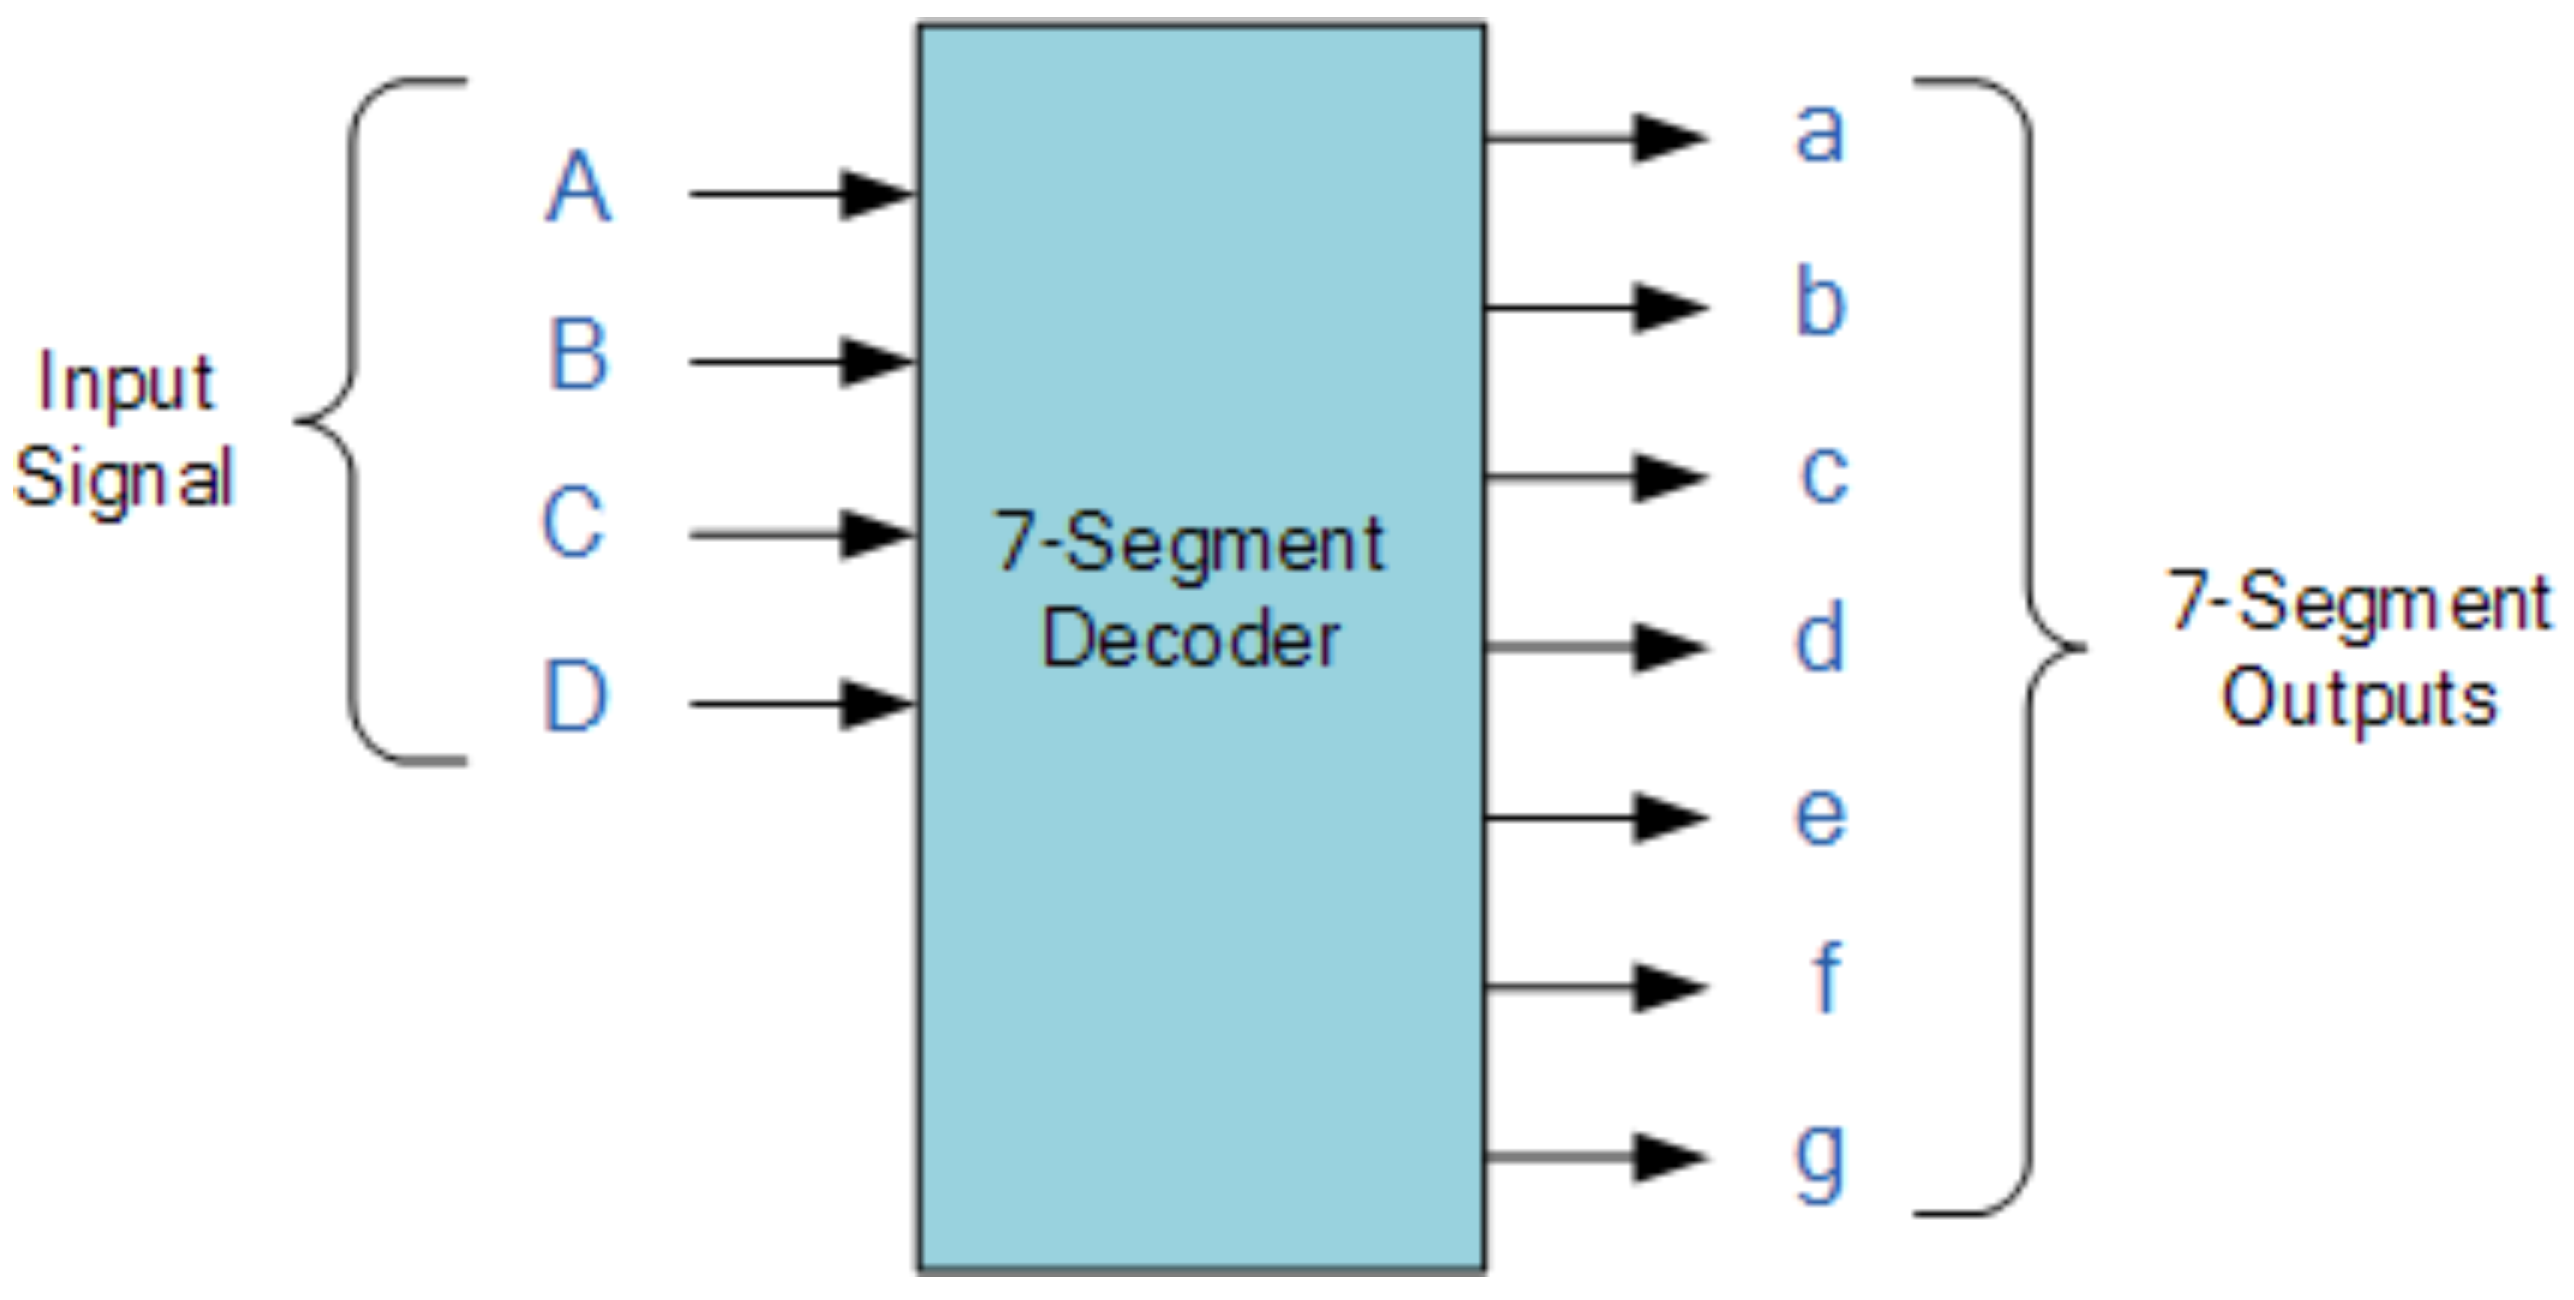
\includegraphics[width=\textwidth]{figs/bcd_7seg.png}
          \captionof*{figure}{Hierum gehts}
        \end{center}
      \column{0.5\textwidth}
      \begin{center}
        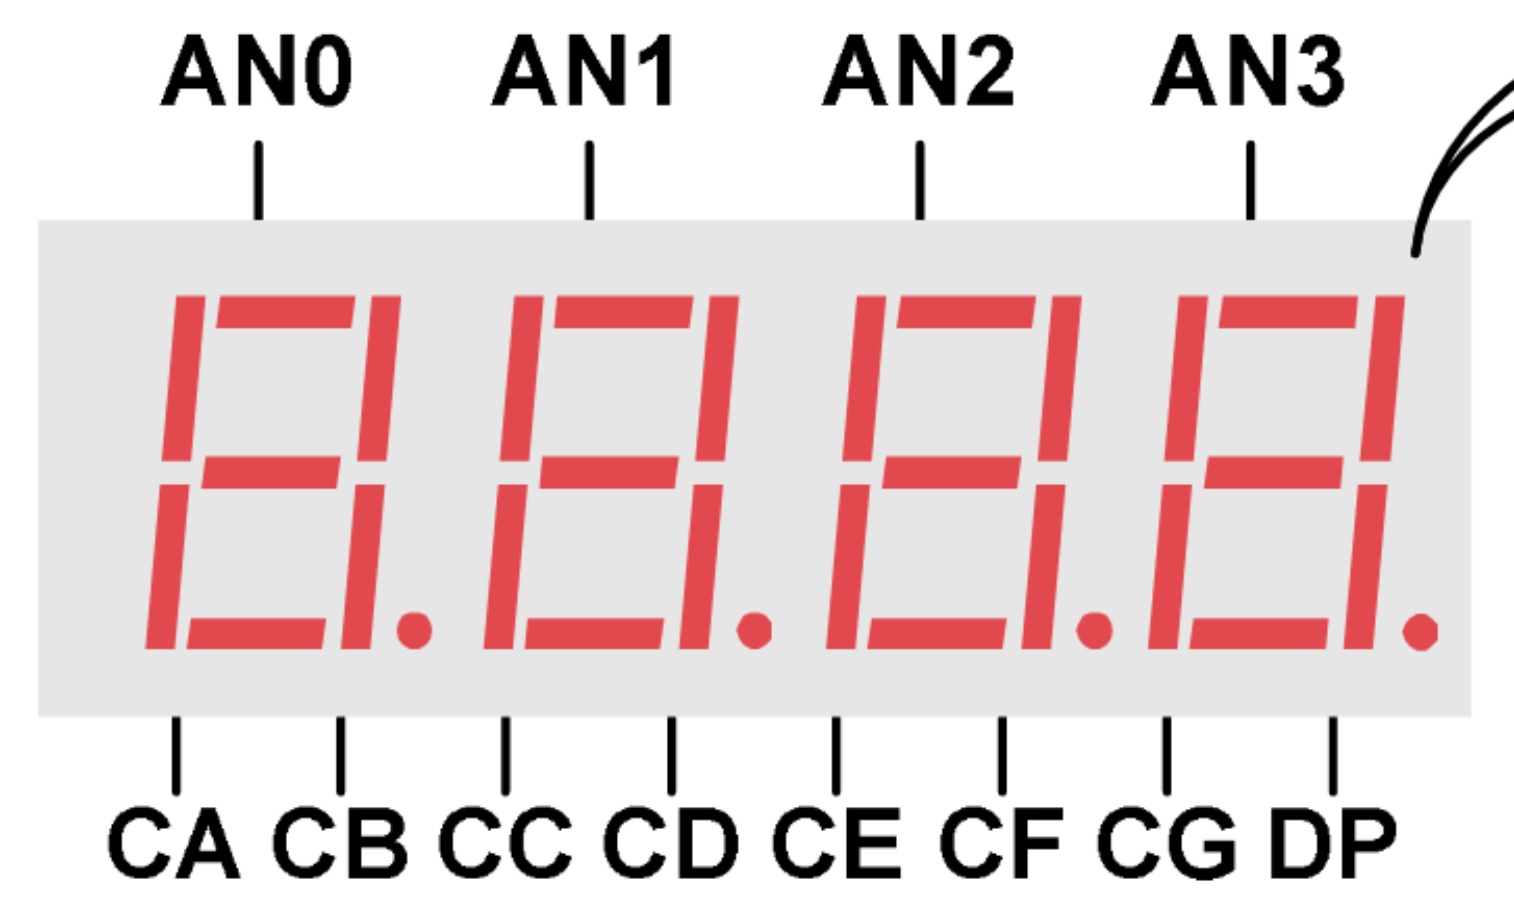
\includegraphics[width=\textwidth]{figs/7seg_package.png}
      \end{center}
    \end{columns}
  \end{frame}

  \begin{frame} [fragile] {Lookuptable (III)}
    \begin{lstlisting}
  case nibVal_v is
    when "0000" => 
      segments_v := "10000001";
    when "0001" => 
      segments_v := "11001111";
    when "0010" => 
      segments_v := "10010010";    
    -- usw
  end case;

  segments_ns <= segments_v;
    \end{lstlisting}
    \begin{alertblock} {}
      Kathode der 7 Seg. Disp. ist low-aktiv.
    \end{alertblock}
  \end{frame}

  %-----------------------------------------------------------------------------
  % ENDE
  %-----------------------------------------------------------------------------

  \section{Ende}
  \begin{frame} {Ende}
    \begin{block} {Nächstes mal}
      \begin{itemize}
        \item Aufgabe 2!
        \item Für die Eiligen:
        \begin{itemize}
          \item Ich versuche heute schon zu Helfen
          \item Sonst immer per Mail erreichbar
        \end{itemize}
      \end{itemize}
    \end{block}
    \begin{exampleblock}{Abschließendes}
      Fragen, Anmerkungen und Verbesserungen ausdrücklich erwünscht.\\
      Ich bin auf euer Feedback angewiesen.
    \end{exampleblock}
  \end{frame}

\end{document}